\begin{figure*}[t]
    \centering
    \begin{minipage}[c]{\textwidth}
    \centering
    \small
    \begin{tabular}{rll}
    \multicolumn{1}{c}{key} & \multicolumn{1}{c}{$p(t)$} & \multicolumn{1}{c}{description} \\ \midrule
         \texttt{`linear\_0'} &  $t \sim \mathcal{U}[0,1]$ & Uniform distribution \\
         \texttt{`linear\_a'} &   $t \sim \frac{1}{1+a}\mathcal{U}[0,1] + \frac{a}{1+a}\delta_1$, where $a \ge 0$ & Uniform distribution w/bias to $t=1$\\
         \texttt{`bias\_t1'} &   $t = g(s)$, $s \sim \mathcal{U}[0,1]$ and $g(s) = \sin\left(s\pi/2)\right)$ & Sine based distribution (bias to $t=1$) \\     
         \texttt{`bias\_t0'} &   $t = g(s)$, $s \sim \mathcal{U}[0,1]$ and $g(s) = \sin\left((s-1)\pi/2)\right) + 1$ & Sine based distribution (bias to $t=0$) \\
         \texttt{`bias\_t0\_t1'} &   $t = g(s)$, with $s \sim \mathcal{U}[0,1]$ and $g(s) = \sin\left(s\pi/2)\right)^2$ & Sine based distribution (bias to $t=1$)   
    \end{tabular}\vspace{.5em}
    
    (a) Different evaluated $p(t)$ training distributions.
    \end{minipage} \vspace{1em}

    \begin{minipage}[c]{.47\textwidth}
    \centering\small
    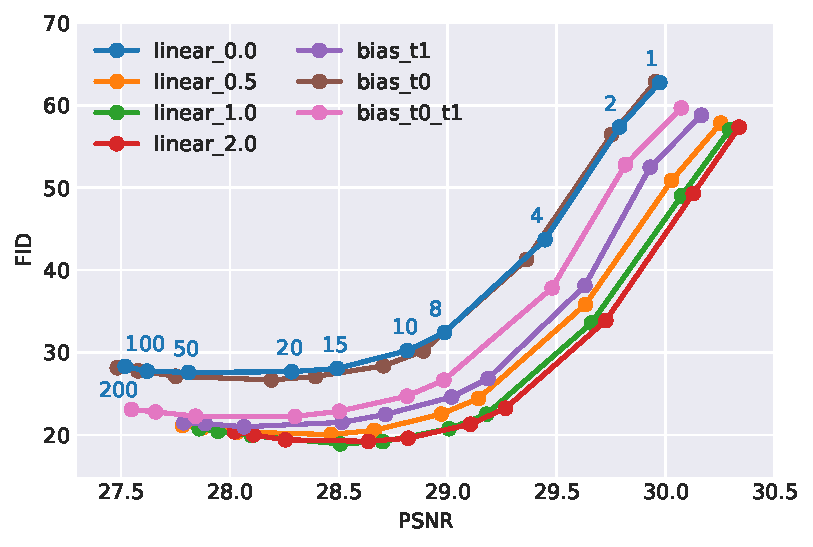
\includegraphics[width=0.9\linewidth]{assets/pd_curve_dejpeg_q15_distro_fid.pdf}
    
    (b) PSNR vs FID plot for different $p(t)$.
    \end{minipage}
    %    
    \begin{minipage}[c]{.47\textwidth}
    \centering\small
    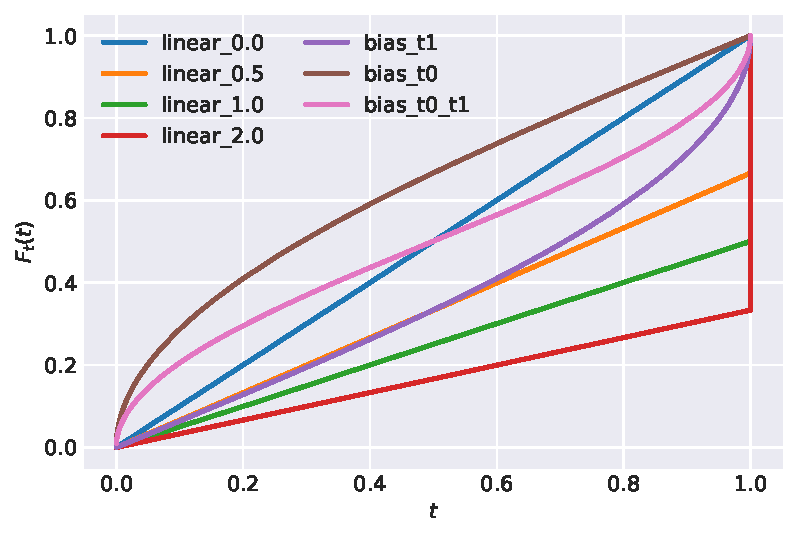
\includegraphics[width=0.9\linewidth]{assets/pd_curve_dejpeg_q15_distro_t.pdf}
    
    (c) Visualization of $p(t)$ cumulative distributions.
    \end{minipage}
    

    \caption{Impact of the distribution of $p(t)$ during training. Results for JPEG Compression removal (Q=15). The best results are obtained when the distribution of $t$ is biased towards $t=1$.}
    \label{fig:dejpeg_distribution_t}
\end{figure*}